\section{Strings}

\subsection{Comandos básicos}

\subsection{Substrings}

\par A função substr de string retorna uma substring interna da string inicial, os parâmetros são:
\begin{itemize}
    \item Posição inicial
    \item Tamanho da substring
\end{itemize}
\par Ex: substring que remove o último char da string str.
\begin{verbatim}
    str.substr(0, str.length()-1);
\end{verbatim}

\subsection{char to int}
\par Para converter um char (i-ésimo char da string) em int, é possível fazer:
\begin{verbatim}
    int x = str[i] - '0';
\end{verbatim}

\subsection{int to string}
\par Para converter um int x em uma string com seus algarismos, fazemos:
\begin{verbatim}
    string str = to_string(x);
\end{verbatim}

\subsection{int to char}
\par Para converter um int x em um char, fazemos:
\begin{verbatim}
    char c = '0' + x;
\end{verbatim}

\subsection{Leitura}
Para se fazer a leitura de uma palavra, pode-se utilizar cin$>>$str. No entanto, 
esse comando não permite a leitura de uma frase, que deve ser feita utilizando 
o comando abaixo
\begin{verbatim}
    getline(cin, s).
\end{verbatim}
Além disso, sempre um cin for utilizado antes do getline, deve-se utilizando o comando
a seguir para "limpar" a entrada
\begin{verbatim}
    cin.ignore()
\end{verbatim}
Desta forma, para uma leitura no estilo t / t frases temos:
\begin{verbatim}
    int t; cin>>t; cin.ignore()
    while (t-->0){
        string str;
        getline(cin, str);
    }
\end{verbatim}
Ademais, para fazer o uso de strings com acento deve-se utilizar os comandos
\begin{verbatim}
    setlocale(LC_ALL, "pt_BR.UTF-8"); wcin; wcout; e wstring;
\end{verbatim}
Não sendo possível utilizar esses comandos separadamente ou com os comandos
básicos do template para C++.

Além disso, também há o comando stringstream, esse que por sua vez tem o objetivo de
receber uma string na construtora e acessar ela palavra/número por palavra/número.
\begin{verbatim}
    string str; getline(cin, str);
    stringstream leitura(str);
    int num;
    while(leitura >> num){nome_vector.push_back(num);}
    //Código que separa todos os números de uma string em um vector.
\end{verbatim}

\subsection{Find}
Dada uma string S e uma substring k, para descobrirmos o índice de início de k em S, 
utilizamos o seguinte comando,
\begin{verbatim}
    int pos = s.find(k);
    if (pos == npos){Não é substring}
\end{verbatim}



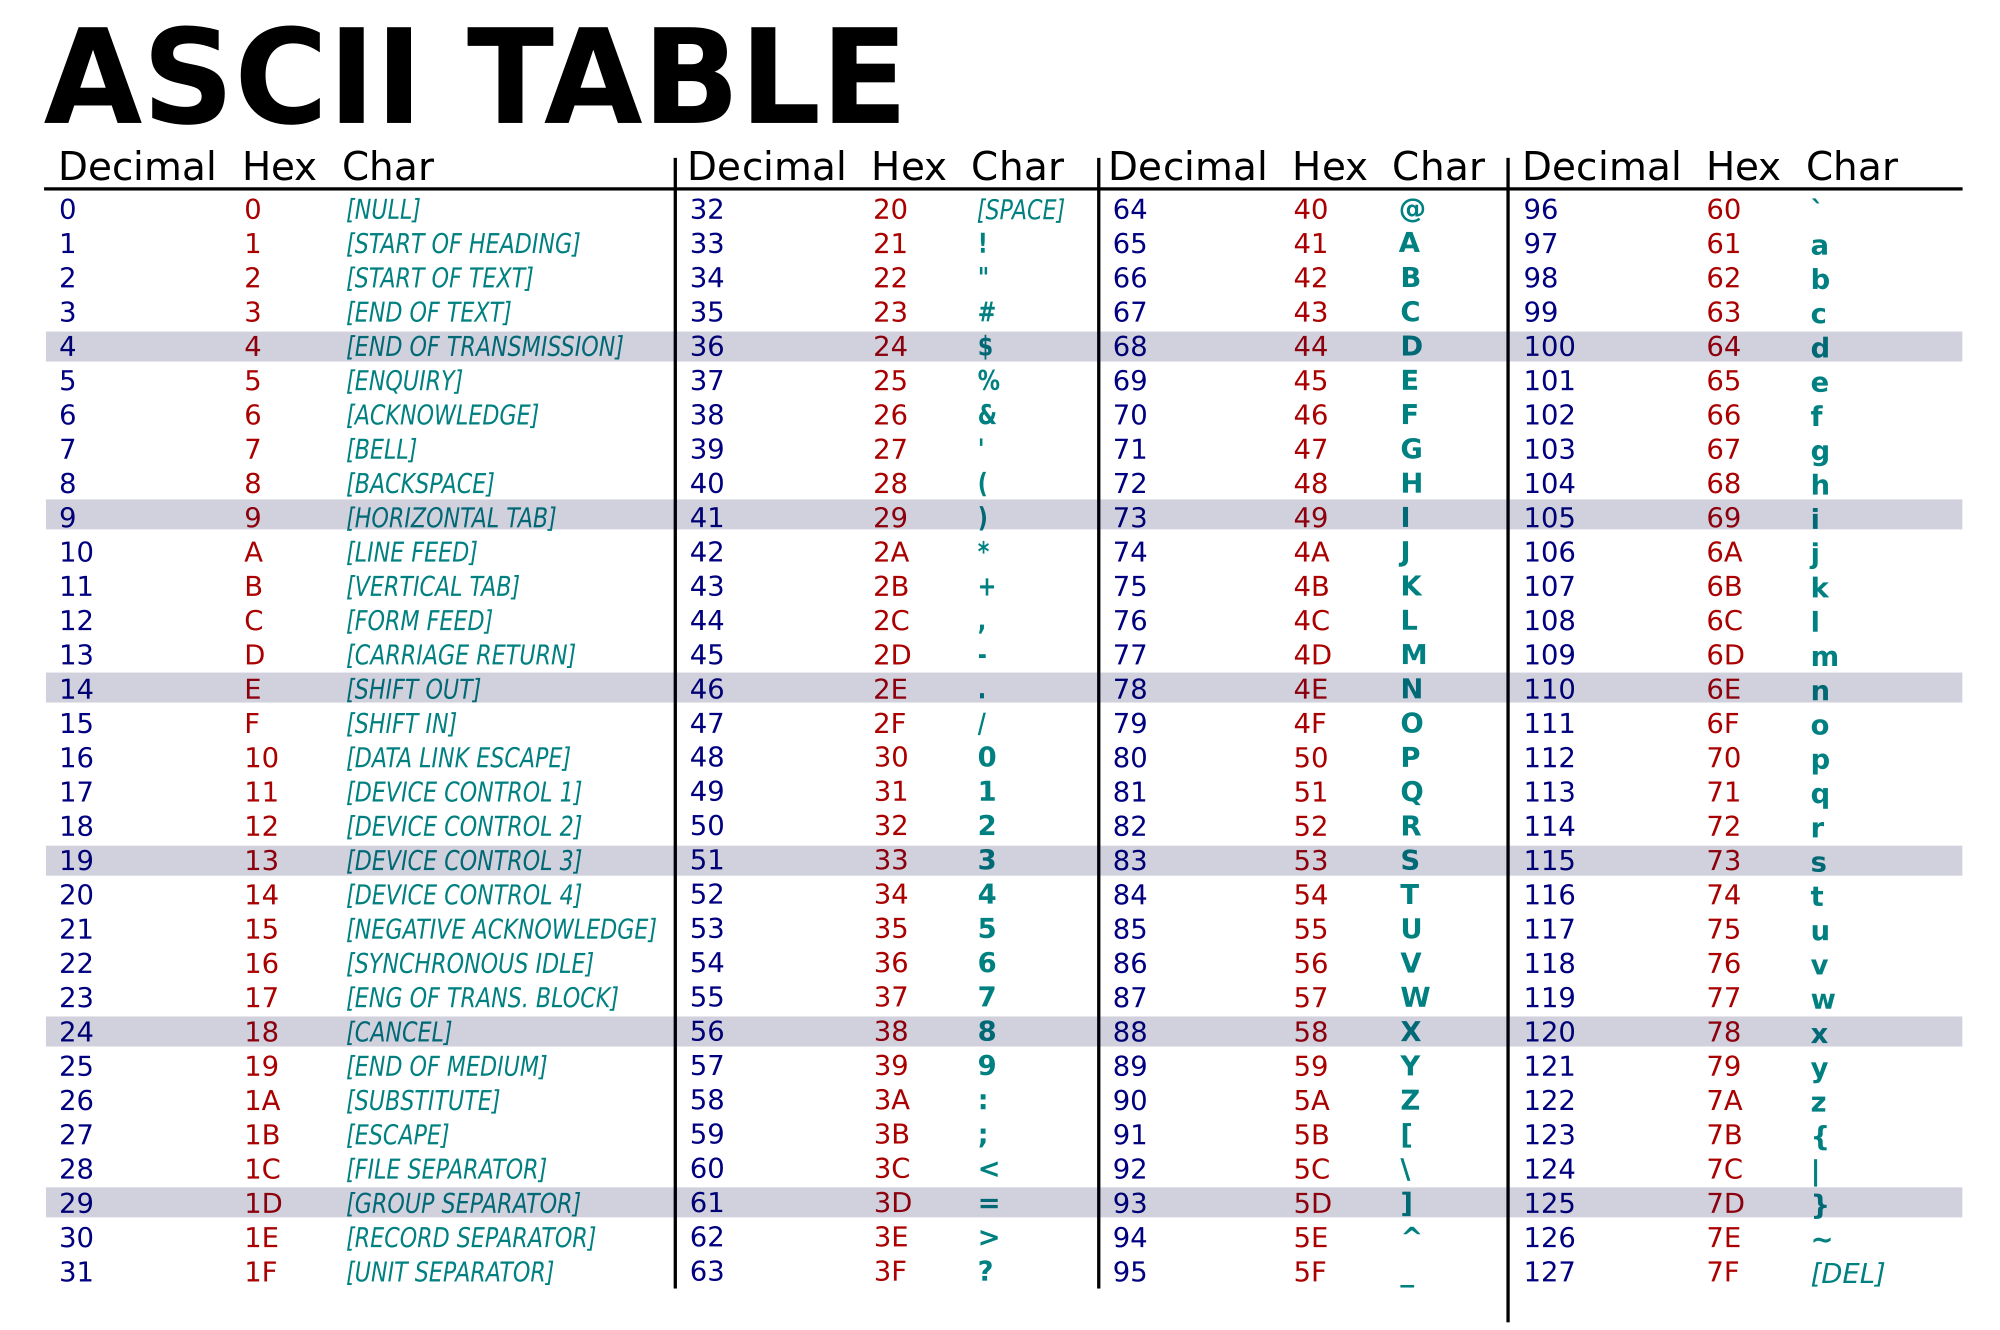
\includegraphics[width=130mm]{6_strings/ASCII.png}
\pagebreak

%%%%%%%%%%%%%%%%%%%%%%%%%%%%%%%%%%%%%%%%%%%%%%%%%%%%%%%%%%%%%%%%%%%%%%%%%%%%%%%%%%%%%%%%%
